\documentclass{article}

\usepackage[utf8]{inputenc}
\usepackage[letterpaper, total={6in, 9in}]{geometry}
\usepackage{amsmath}
\usepackage{natbib}
\usepackage{wrapfig}
\usepackage{graphicx}
\usepackage{amssymb}
\usepackage{tikz}

\graphicspath{ {./geo2/} }


\title{Geometry 2 - Circles}
\author{TSS Math Club}
\date{Oct 2022}

\begin{document}
\large

\maketitle

\section{Basic property of Circles}
\subsection{Definition of Circles}
\subsection{Terms to describe geometric object related to circles}

\begin{minipage}{.7\linewidth}
\begin{itemize}
  \item Center: Point O.
  \item Radius: Length from center to perimeter.
  \item Arc: A curved line on the circumference of a circle.
  \item Chord: A straight line between two points on a circle.
  \item Central angle: \(\angle BOC\) would be an example of a central angle.
  \item Inscribed angle: \(\angle BAC\) would be an example of an inscribed angle.
\end{itemize}
\end{minipage}
\hfill
\begin{minipage}{.3\linewidth}
\tikzset{every picture/.style={line width=0.75pt}} %set default line width to 0.75pt        
    
    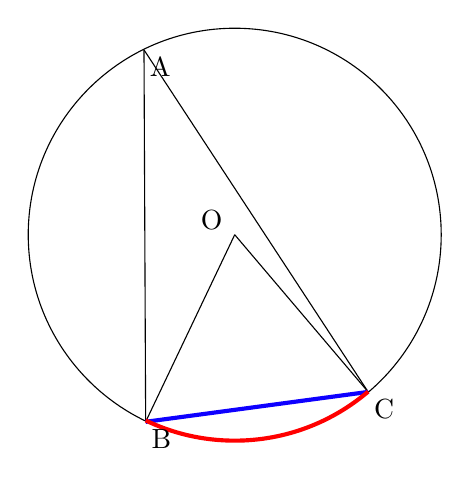
\begin{tikzpicture}[x=0.75pt,y=0.75pt,yscale=-0.8,xscale=0.8]
        %uncomment if require: \path (0,300); %set diagram left start at 0, and has height of 300
        
        %Shape: Circle [id:dp17379134999161217] 
        \draw   (28,148.36) .. controls (28,79.68) and (83.68,24) .. (152.36,24) .. controls (221.04,24) and (276.72,79.68) .. (276.72,148.36) .. controls (276.72,217.04) and (221.04,272.72) .. (152.36,272.72) .. controls (83.68,272.72) and (28,217.04) .. (28,148.36) -- cycle ;
        %Straight Lines [id:da45878936702265327] 
        \draw    (152.36,148.36) -- (232.72,243.03) ;
        %Straight Lines [id:da6953334630723775] 
        \draw    (152.36,148.36) -- (98.72,261.03) ;
        %Straight Lines [id:da21878844711573953] 
        \draw    (97.72,37.03) -- (98.72,261.03) ;
        %Straight Lines [id:da3182172562914929] 
        \draw    (97.72,37.03) -- (232.72,243.03) ;
        %Straight Lines [id:da9967812564105096] 
        \draw [color={rgb, 255:red, 14; green, 0; blue, 255 }  ,draw opacity=1 ][line width=1.5]    (98.72,261.03) -- (232.72,243.03) ;
        %Shape: Arc [id:dp9816832896319678] 
        \draw  [draw opacity=0][line width=1.5]  (232.73,242.82) .. controls (211.08,261.25) and (183.02,272.38) .. (152.36,272.38) .. controls (133.15,272.38) and (114.96,268.01) .. (98.72,260.21) -- (152.36,148.36) -- cycle ; \draw  [color={rgb, 255:red, 255; green, 0; blue, 0 }  ,draw opacity=1 ][line width=1.5]  (232.73,242.82) .. controls (211.08,261.25) and (183.02,272.38) .. (152.36,272.38) .. controls (133.15,272.38) and (114.96,268.01) .. (98.72,260.21) ;  
        
        % Text Node
        \draw (130.36,132.36) node [anchor=north west][inner sep=0.75pt]   [align=left] {O};
        % Text Node
        \draw (99.72,40.03) node [anchor=north west][inner sep=0.75pt]   [align=left] {A};
        % Text Node
        \draw (100.72,264.03) node [anchor=north west][inner sep=0.75pt]   [align=left] {B};
        % Text Node
        \draw (234.72,246.03) node [anchor=north west][inner sep=0.75pt]   [align=left] {C};
        
        
    \end{tikzpicture}
\end{minipage}

\subsection{Central angle is twice any inscribed angle}


\begin{minipage}{.2\linewidth}
\tikzset{every picture/.style={line width=0.75pt}} %set default line width to 0.75pt        

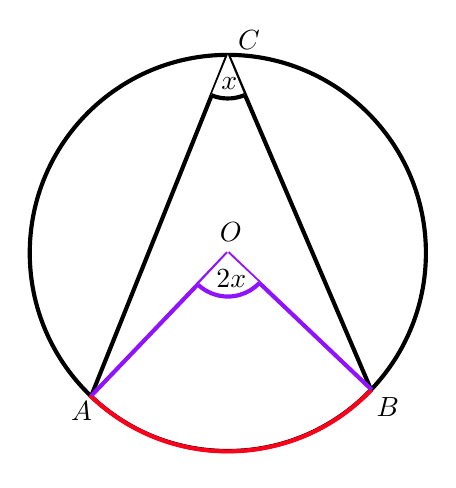
\begin{tikzpicture}[x=0.75pt,y=0.75pt,yscale=-0.7,xscale=0.7]
%uncomment if require: \path (0,419); %set diagram left start at 0, and has height of 419

%Shape: Circle [id:dp5403186956911956] 
\draw  [line width=1.5]  (203.33,174.67) .. controls (203.33,99.37) and (264.37,38.33) .. (339.67,38.33) .. controls (414.96,38.33) and (476,99.37) .. (476,174.67) .. controls (476,249.96) and (414.96,311) .. (339.67,311) .. controls (264.37,311) and (203.33,249.96) .. (203.33,174.67) -- cycle ;
%Straight Lines [id:da5957136609895495] 
\draw [color={rgb, 255:red, 0; green, 0; blue, 0 }  ,draw opacity=1 ][fill={rgb, 255:red, 255; green, 255; blue, 255 }  ,fill opacity=1 ][line width=1.5]    (339.67,38.33) -- (438.33,269) ;
%Straight Lines [id:da6339312134822053] 
\draw [color={rgb, 255:red, 0; green, 0; blue, 0 }  ,draw opacity=1 ][fill={rgb, 255:red, 255; green, 255; blue, 255 }  ,fill opacity=1 ][line width=1.5]    (339.67,38.33) -- (245.67,273) ;
%Shape: Arc [id:dp5366702840230211] 
\draw  [draw opacity=0][fill={rgb, 255:red, 255; green, 255; blue, 255 }  ,fill opacity=1 ][line width=1.5]  (351.17,66.04) .. controls (345.14,68.55) and (338.25,69.12) .. (331.48,67.2) .. controls (330.39,66.88) and (329.32,66.52) .. (328.29,66.09) -- (339.67,38.33) -- cycle ; \draw  [color={rgb, 255:red, 0; green, 0; blue, 0 }  ,draw opacity=1 ][line width=1.5]  (351.17,66.04) .. controls (345.14,68.55) and (338.25,69.12) .. (331.48,67.2) .. controls (330.39,66.88) and (329.32,66.52) .. (328.29,66.09) ;  
%Shape: Arc [id:dp9498591182227187] 
\draw  [draw opacity=0][line width=1.5]  (438.55,268.73) .. controls (417.51,290.96) and (388.92,306.26) .. (356.19,310.24) .. controls (313.61,315.44) and (273.22,300.36) .. (244.66,272.57) -- (339.67,174.67) -- cycle ; \draw  [color={rgb, 255:red, 255; green, 0; blue, 27 }  ,draw opacity=1 ][line width=1.5]  (438.55,268.73) .. controls (417.51,290.96) and (388.92,306.26) .. (356.19,310.24) .. controls (313.61,315.44) and (273.22,300.36) .. (244.66,272.57) ;  
%Straight Lines [id:da06768614777660997] 
\draw [color={rgb, 255:red, 144; green, 19; blue, 254 }  ,draw opacity=1 ][line width=1.5]    (339.67,174.67) -- (245.67,273) ;
%Straight Lines [id:da712391157904465] 
\draw [color={rgb, 255:red, 144; green, 19; blue, 254 }  ,draw opacity=1 ][line width=1.5]    (339.67,174.67) -- (438.55,268.73) ;
%Shape: Arc [id:dp1573251124672308] 
\draw  [draw opacity=0][fill={rgb, 255:red, 255; green, 255; blue, 255 }  ,fill opacity=1 ][line width=1.5]  (361.51,195.24) .. controls (354.08,203.12) and (342.62,206.69) .. (331.48,203.53) .. controls (326.7,202.17) and (322.52,199.73) .. (319.14,196.55) -- (339.67,174.67) -- cycle ; \draw  [color={rgb, 255:red, 144; green, 19; blue, 254 }  ,draw opacity=1 ][line width=1.5]  (361.51,195.24) .. controls (354.08,203.12) and (342.62,206.69) .. (331.48,203.53) .. controls (326.7,202.17) and (322.52,199.73) .. (319.14,196.55) ;  

% Text Node
\draw (333.33,52.07) node [anchor=north west][inner sep=0.75pt]    {$x$};
% Text Node
\draw (230,275.4) node [anchor=north west][inner sep=0.75pt]    {$A$};
% Text Node
\draw (440.33,272.4) node [anchor=north west][inner sep=0.75pt]    {$B$};
% Text Node
\draw (330,184.4) node [anchor=north west][inner sep=0.75pt]    {$2x$};
% Text Node
\draw (332.33,152.07) node [anchor=north west][inner sep=0.75pt]    {$O$};
% Text Node
\draw (345,20) node [anchor=north west][inner sep=0.75pt]    {$C$};

\end{tikzpicture}
\end{minipage}
\hfill
\begin{minipage}{.6\linewidth}

Create a line from point C that goes through point O and hits the circumference of the circle. Name this point P, and label \(\angle ACO\) as \(y\).\\
Since triangle \(\triangle COA\) is an isosceles (\(CO=AO\)), \(\angle ACO\) and \(\angle CAO\) are the same, and thus \(\angle AOP\) is equal to \(2y\).\\
Label \(\angle BCO\) as \(z\), and since \(\triangle COB\) is also an isosceles triangle, \(\angle BOC\) is equivalent to \(2z\).\\
Therefore, \(\angle AOB=2y+2z=2y+z=2x\). 

\end{minipage}



\pagebreak

\subsection{Inscribed angles subtended by the same arc are equal}


\begin{minipage}{0.3\linewidth}
\tikzset{every picture/.style={line width=0.75pt}} %set default line width to 0.75pt        

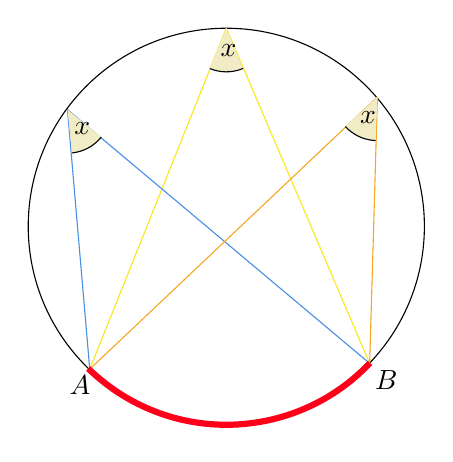
\begin{tikzpicture}[x=0.75pt,y=0.75pt,yscale=-0.7,xscale=0.7]
%uncomment if require: \path (0,419); %set diagram left start at 0, and has height of 419

%Shape: Circle [id:dp5403186956911956] 
\draw   (203.33,174.67) .. controls (203.33,99.37) and (264.37,38.33) .. (339.67,38.33) .. controls (414.96,38.33) and (476,99.37) .. (476,174.67) .. controls (476,249.96) and (414.96,311) .. (339.67,311) .. controls (264.37,311) and (203.33,249.96) .. (203.33,174.67) -- cycle ;
%Straight Lines [id:da5957136609895495] 
\draw [color={rgb, 255:red, 248; green, 231; blue, 28 }  ,draw opacity=1 ][fill={rgb, 255:red, 241; green, 236; blue, 197 }  ,fill opacity=1 ]   (339.67,38.33) -- (438.33,269) ;
%Straight Lines [id:da33122143131158555] 
\draw [color={rgb, 255:red, 74; green, 144; blue, 226 }  ,draw opacity=1 ][fill={rgb, 255:red, 241; green, 236; blue, 197 }  ,fill opacity=1 ]   (230.33,94.33) -- (245.67,273) ;
%Straight Lines [id:da6339312134822053] 
\draw [color={rgb, 255:red, 248; green, 231; blue, 28 }  ,draw opacity=1 ][fill={rgb, 255:red, 241; green, 236; blue, 197 }  ,fill opacity=1 ]   (339.67,38.33) -- (245.67,273) ;
%Straight Lines [id:da8938383138384509] 
\draw [color={rgb, 255:red, 74; green, 144; blue, 226 }  ,draw opacity=1 ][fill={rgb, 255:red, 241; green, 236; blue, 197 }  ,fill opacity=1 ]   (230.33,94.33) -- (267.33,125.4) -- (438.33,269) ;
%Straight Lines [id:da24326554605856554] 
\draw [color={rgb, 255:red, 245; green, 166; blue, 35 }  ,draw opacity=1 ][fill={rgb, 255:red, 241; green, 236; blue, 197 }  ,fill opacity=1 ]   (245.67,273) -- (443.67,85.67) ;
%Straight Lines [id:da9944164254362617] 
\draw [color={rgb, 255:red, 245; green, 166; blue, 35 }  ,draw opacity=1 ][fill={rgb, 255:red, 241; green, 236; blue, 197 }  ,fill opacity=1 ]   (443.67,85.67) -- (438.33,269) ;
%Shape: Arc [id:dp2640858128507122] 
\draw  [draw opacity=0][fill={rgb, 255:red, 241; green, 236; blue, 197 }  ,fill opacity=1 ] (253.62,113.25) .. controls (249.5,118.32) and (243.71,122.09) .. (236.84,123.62) .. controls (235.73,123.87) and (234.61,124.05) .. (233.51,124.17) -- (230.33,94.33) -- cycle ; \draw   (253.62,113.25) .. controls (249.5,118.32) and (243.71,122.09) .. (236.84,123.62) .. controls (235.73,123.87) and (234.61,124.05) .. (233.51,124.17) ;  
%Shape: Arc [id:dp5366702840230211] 
\draw  [draw opacity=0][fill={rgb, 255:red, 241; green, 236; blue, 197 }  ,fill opacity=1 ] (351.17,66.04) .. controls (345.14,68.55) and (338.25,69.12) .. (331.48,67.2) .. controls (330.39,66.88) and (329.32,66.52) .. (328.29,66.09) -- (339.67,38.33) -- cycle ; \draw   (351.17,66.04) .. controls (345.14,68.55) and (338.25,69.12) .. (331.48,67.2) .. controls (330.39,66.88) and (329.32,66.52) .. (328.29,66.09) ;  
%Shape: Arc [id:dp5386457051908322] 
\draw  [draw opacity=0][fill={rgb, 255:red, 241; green, 236; blue, 197 }  ,fill opacity=1 ] (442.39,115.64) .. controls (435.86,115.37) and (429.38,112.97) .. (424.06,108.37) .. controls (423.19,107.62) and (422.38,106.84) .. (421.62,106.02) -- (443.67,85.67) -- cycle ; \draw   (442.39,115.64) .. controls (435.86,115.37) and (429.38,112.97) .. (424.06,108.37) .. controls (423.19,107.62) and (422.38,106.84) .. (421.62,106.02) ;  
%Shape: Arc [id:dp9498591182227187] 
\draw  [draw opacity=0][line width=2.25]  (438.55,268.73) .. controls (417.51,290.96) and (388.92,306.26) .. (356.19,310.24) .. controls (313.61,315.44) and (273.22,300.36) .. (244.66,272.57) -- (339.67,174.67) -- cycle ; \draw  [color={rgb, 255:red, 255; green, 0; blue, 27 }  ,draw opacity=1 ][line width=2.25]  (438.55,268.73) .. controls (417.51,290.96) and (388.92,306.26) .. (356.19,310.24) .. controls (313.61,315.44) and (273.22,300.36) .. (244.66,272.57) ;  

% Text Node
\draw (233.33,101.4) node [anchor=north west][inner sep=0.75pt]    {$x$};
% Text Node
\draw (334,48.07) node [anchor=north west][inner sep=0.75pt]    {$x$};
% Text Node
\draw (430,94.07) node [anchor=north west][inner sep=0.75pt]    {$x$};
% Text Node
\draw (230,275.4) node [anchor=north west][inner sep=0.75pt]    {$A$};
% Text Node
\draw (440.33,272.4) node [anchor=north west][inner sep=0.75pt]    {$B$};

\end{tikzpicture}
\end{minipage}
\hfill
\begin{minipage}{0.6\linewidth}
Since an inscribed angle is half of its center angle with the same arc (ref 1.3), and all three angles share the same arc, the inscribed angles are all equal.
\end{minipage}

\vspace{140px}

\subsection{Angle subtended by a diameter is \(90^{\circ}\)}

\begin{minipage}{0.5\linewidth}

\tikzset{every picture/.style={line width=0.75pt}} %set default line width to 0.75pt        

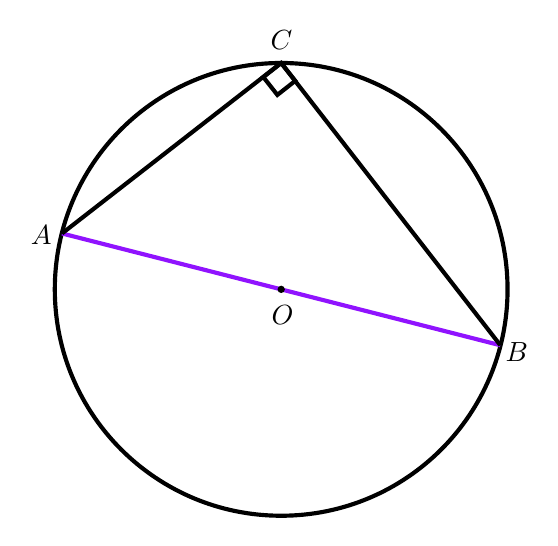
\begin{tikzpicture}[x=0.75pt,y=0.75pt,yscale=-.8,xscale=.8]
%uncomment if require: \path (0,419); %set diagram left start at 0, and has height of 419

%Shape: Circle [id:dp5403186956911956] 
\draw  [line width=1.5]  (203.33,174.67) .. controls (203.33,99.37) and (264.37,38.33) .. (339.67,38.33) .. controls (414.96,38.33) and (476,99.37) .. (476,174.67) .. controls (476,249.96) and (414.96,311) .. (339.67,311) .. controls (264.37,311) and (203.33,249.96) .. (203.33,174.67) -- cycle ;
%Straight Lines [id:da06811875685737068] 
\draw [color={rgb, 255:red, 144; green, 19; blue, 254 }  ,draw opacity=1 ][line width=1.5]    (339.67,174.67) -- (471.67,208.33) ;
%Straight Lines [id:da4067465378250854] 
\draw [color={rgb, 255:red, 144; green, 19; blue, 254 }  ,draw opacity=1 ][line width=1.5]    (207.67,141) -- (339.67,174.67) ;
%Straight Lines [id:da6912410596897796] 
\draw [line width=1.5]    (339.67,38.33) -- (471.67,208.33) ;
%Straight Lines [id:da8601096491144575] 
\draw [line width=1.5]    (339.67,38.33) -- (207.67,141) ;
%Shape: Square [id:dp24268413759610286] 
\draw  [line width=1.5]  (328.91,46.8) -- (339.67,38.33) -- (348.14,49.09) -- (337.38,57.56) -- cycle ;
%Shape: Circle [id:dp8767343798761416] 
\draw  [fill={rgb, 255:red, 0; green, 0; blue, 0 }  ,fill opacity=1 ] (337.83,174.67) .. controls (337.83,173.65) and (338.65,172.83) .. (339.67,172.83) .. controls (340.68,172.83) and (341.5,173.65) .. (341.5,174.67) .. controls (341.5,175.68) and (340.68,176.5) .. (339.67,176.5) .. controls (338.65,176.5) and (337.83,175.68) .. (337.83,174.67) -- cycle ;

% Text Node
\draw (187.33,134.4) node [anchor=north west][inner sep=0.75pt]    {$A$};
% Text Node
\draw (473.33,205.07) node [anchor=north west][inner sep=0.75pt]    {$B$};
% Text Node
\draw (331.67,17.4) node [anchor=north west][inner sep=0.75pt]    {$C$};
% Text Node
\draw (332.33,183.07) node [anchor=north west][inner sep=0.75pt]    {$O$};


\end{tikzpicture}
\end{minipage}
\hfill
\begin{minipage}{0.5\linewidth}
Both angles share the same arc, thus $\angle ACB$ is half of $\angle AOB$ $90^{\circ}$ is half of $180^{\circ}$.
\end{minipage}


\pagebreak

\subsection{Perpendicular chord theorem}

\begin{minipage}{0.4\linewidth}

\tikzset{every picture/.style={line width=0.75pt}} %set default line width to 0.75pt        

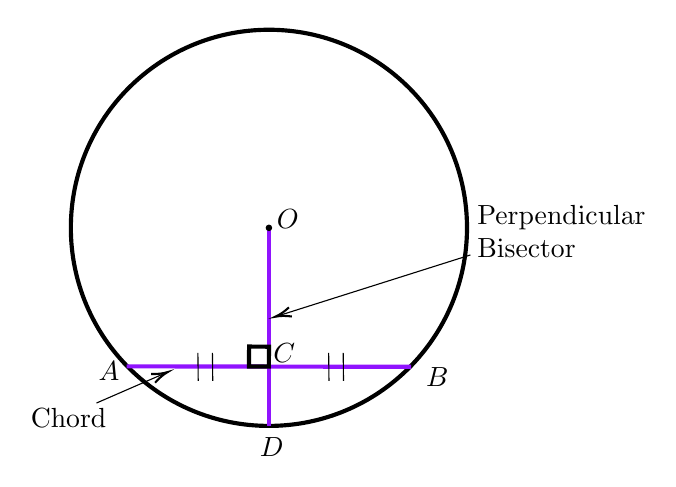
\begin{tikzpicture}[x=0.75pt,y=0.75pt,yscale=-.7,xscale=.7]
%uncomment if require: \path (0,419); %set diagram left start at 0, and has height of 419

%Shape: Circle [id:dp5403186956911956] 
\draw  [line width=1.5]  (203.33,174.67) .. controls (203.33,99.37) and (264.37,38.33) .. (339.67,38.33) .. controls (414.96,38.33) and (476,99.37) .. (476,174.67) .. controls (476,249.96) and (414.96,311) .. (339.67,311) .. controls (264.37,311) and (203.33,249.96) .. (203.33,174.67) -- cycle ;
%Straight Lines [id:da06811875685737068] 
\draw [color={rgb, 255:red, 144; green, 19; blue, 254 }  ,draw opacity=1 ][line width=1.5]    (241.67,270) -- (437.56,270.33) ;
%Straight Lines [id:da4067465378250854] 
\draw [color={rgb, 255:red, 144; green, 19; blue, 254 }  ,draw opacity=1 ][line width=1.5]    (339.67,311) -- (339.67,174.67) ;
%Shape: Circle [id:dp8767343798761416] 
\draw  [fill={rgb, 255:red, 0; green, 0; blue, 0 }  ,fill opacity=1 ] (337.83,174.67) .. controls (337.83,173.65) and (338.65,172.83) .. (339.67,172.83) .. controls (340.68,172.83) and (341.5,173.65) .. (341.5,174.67) .. controls (341.5,175.68) and (340.68,176.5) .. (339.67,176.5) .. controls (338.65,176.5) and (337.83,175.68) .. (337.83,174.67) -- cycle ;
%Shape: Square [id:dp7558142713797231] 
\draw  [line width=1.5]  (326.02,256.38) -- (339.71,256.48) -- (339.61,270.17) -- (325.92,270.07) -- cycle ;
%Straight Lines [id:da40971348906843996] 
\draw    (300.78,260.67) -- (301,280) ;
%Straight Lines [id:da8507674313612943] 
\draw    (290.78,260.67) -- (291,280) ;
%Straight Lines [id:da007449580833429614] 
\draw    (390.78,260.67) -- (391,280) ;
%Straight Lines [id:da4940931408813922] 
\draw    (380.78,260.67) -- (381,280) ;

% Text Node
\draw (481.33,157.22) node [anchor=north west][inner sep=0.75pt]   [align=left] {Perpendicular \\Bisector};
% Text Node
\draw (330,229.56) node [anchor=north west][inner sep=0.75pt]   [align=left] { };
% Text Node
\draw (174,297.11) node [anchor=north west][inner sep=0.75pt]   [align=left] {Chord};
% Text Node
\draw (273,261.22) node [anchor=north west][inner sep=0.75pt]   [align=left] { };
% Text Node
\draw (343.33,160.07) node [anchor=north west][inner sep=0.75pt]    {$O$};
% Text Node
\draw (220.67,264.96) node [anchor=north west][inner sep=0.75pt]    {$A$};
% Text Node
\draw (446,269.29) node [anchor=north west][inner sep=0.75pt]    {$B$};
% Text Node
\draw (341,252.62) node [anchor=north west][inner sep=0.75pt]    {$C$};
% Text Node
\draw (331.67,317.29) node [anchor=north west][inner sep=0.75pt]    {$D$};
% Connection
\draw    (478.33,193.34) -- (345.91,235.26) ;
\draw [shift={(344,235.86)}, rotate = 342.43] [color={rgb, 255:red, 0; green, 0; blue, 0 }  ][line width=0.75]    (10.93,-3.29) .. controls (6.95,-1.4) and (3.31,-0.3) .. (0,0) .. controls (3.31,0.3) and (6.95,1.4) .. (10.93,3.29)   ;
% Connection
\draw    (221,295.24) -- (268.17,274.72) ;
\draw [shift={(270,273.92)}, rotate = 156.49] [color={rgb, 255:red, 0; green, 0; blue, 0 }  ][line width=0.75]    (10.93,-3.29) .. controls (6.95,-1.4) and (3.31,-0.3) .. (0,0) .. controls (3.31,0.3) and (6.95,1.4) .. (10.93,3.29)   ;

\end{tikzpicture}
\end{minipage}
\hfill
\begin{minipage}{0.425\linewidth}

Connect point A to O, and point O to B. Note: AO and BO are both the radii of the circle.
As a result, $\triangle AOC$ and $\triangle BOC$ are congruent triangles, with $AB=CB$. Therefore, the radius bisects AB.
\end{minipage}

\vspace{50px}

\subsection{Tangent to a circle}

\subsubsection{Definition}

A line that intersects a circle at only one point.

\subsubsection{The radius from the center of the circle to the point of tangency is perpendicular to the tangent line}
\begin{minipage}{0.2\linewidth}
\tikzset{every picture/.style={line width=0.75pt}} %set default line width to 0.75pt        

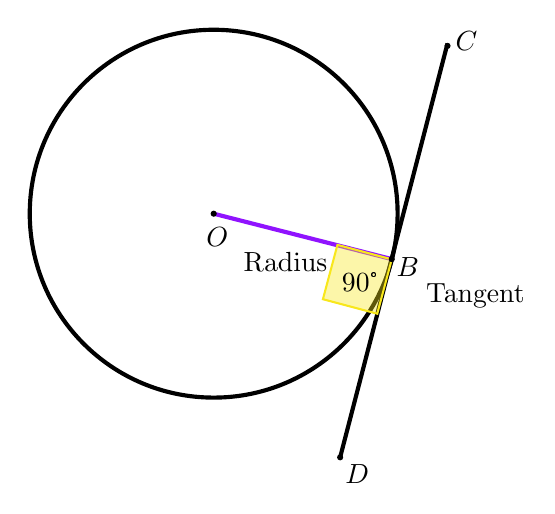
\begin{tikzpicture}[x=0.75pt,y=0.75pt,yscale=-0.65,xscale=0.65]
%uncomment if require: \path (0,419); %set diagram left start at 0, and has height of 419

%Shape: Circle [id:dp5403186956911956] 
\draw  [line width=1.5]  (203.33,174.67) .. controls (203.33,99.37) and (264.37,38.33) .. (339.67,38.33) .. controls (414.96,38.33) and (476,99.37) .. (476,174.67) .. controls (476,249.96) and (414.96,311) .. (339.67,311) .. controls (264.37,311) and (203.33,249.96) .. (203.33,174.67) -- cycle ;
%Straight Lines [id:da06811875685737068] 
\draw [color={rgb, 255:red, 144; green, 19; blue, 254 }  ,draw opacity=1 ][line width=1.5]    (339.67,174.67) -- (471.67,208.33) ;
%Shape: Circle [id:dp8767343798761416] 
\draw  [fill={rgb, 255:red, 0; green, 0; blue, 0 }  ,fill opacity=1 ] (337.83,174.67) .. controls (337.83,173.65) and (338.65,172.83) .. (339.67,172.83) .. controls (340.68,172.83) and (341.5,173.65) .. (341.5,174.67) .. controls (341.5,175.68) and (340.68,176.5) .. (339.67,176.5) .. controls (338.65,176.5) and (337.83,175.68) .. (337.83,174.67) -- cycle ;
%Straight Lines [id:da10641417010205423] 
\draw [line width=1.5]    (433.4,355.27) -- (513,48.47) ;
%Shape: Square [id:dp24268413759610286] 
\draw  [color={rgb, 255:red, 248; green, 231; blue, 28 }  ,draw opacity=1 ][fill={rgb, 255:red, 248; green, 231; blue, 28 }  ,fill opacity=0.38 ][line width=0.75]  (431.39,197.78) -- (471.67,208.53) -- (460.91,248.81) -- (420.64,238.06) -- cycle ;
%Shape: Circle [id:dp49749378737218897] 
\draw  [fill={rgb, 255:red, 0; green, 0; blue, 0 }  ,fill opacity=1 ] (469.83,208.33) .. controls (469.83,207.32) and (470.65,206.5) .. (471.67,206.5) .. controls (472.68,206.5) and (473.5,207.32) .. (473.5,208.33) .. controls (473.5,209.35) and (472.68,210.17) .. (471.67,210.17) .. controls (470.65,210.17) and (469.83,209.35) .. (469.83,208.33) -- cycle ;
%Shape: Circle [id:dp7955108597985465] 
\draw  [fill={rgb, 255:red, 0; green, 0; blue, 0 }  ,fill opacity=1 ] (431.57,355.27) .. controls (431.57,354.25) and (432.39,353.43) .. (433.4,353.43) .. controls (434.41,353.43) and (435.23,354.25) .. (435.23,355.27) .. controls (435.23,356.28) and (434.41,357.1) .. (433.4,357.1) .. controls (432.39,357.1) and (431.57,356.28) .. (431.57,355.27) -- cycle ;
%Shape: Circle [id:dp0003285569832827129] 
\draw  [fill={rgb, 255:red, 0; green, 0; blue, 0 }  ,fill opacity=1 ] (511.17,50.3) .. controls (511.17,49.29) and (511.99,48.47) .. (513,48.47) .. controls (514.01,48.47) and (514.83,49.29) .. (514.83,50.3) .. controls (514.83,51.31) and (514.01,52.13) .. (513,52.13) .. controls (511.99,52.13) and (511.17,51.31) .. (511.17,50.3) -- cycle ;

% Text Node
\draw (473.33,205.07) node [anchor=north west][inner sep=0.75pt]    {$B$};
% Text Node
\draw (517,37.87) node [anchor=north west][inner sep=0.75pt]    {$C$};
% Text Node
\draw (332.33,183.07) node [anchor=north west][inner sep=0.75pt]    {$O$};
% Text Node
\draw (435.4,358.67) node [anchor=north west][inner sep=0.75pt]    {$D$};
% Text Node
\draw (360,201.07) node [anchor=north west][inner sep=0.75pt]   [align=left] {Radius};
% Text Node
\draw (495.2,224.47) node [anchor=north west][inner sep=0.75pt]   [align=left] {Tangent};
% Text Node
\draw (432.8,216.07) node [anchor=north west][inner sep=0.75pt]   [align=left] {90°};


\end{tikzpicture}
\end{minipage}
\hfill
\begin{minipage}{0.4\linewidth}

\tikzset{every picture/.style={line width=0.75pt}} %set default line width to 0.75pt        

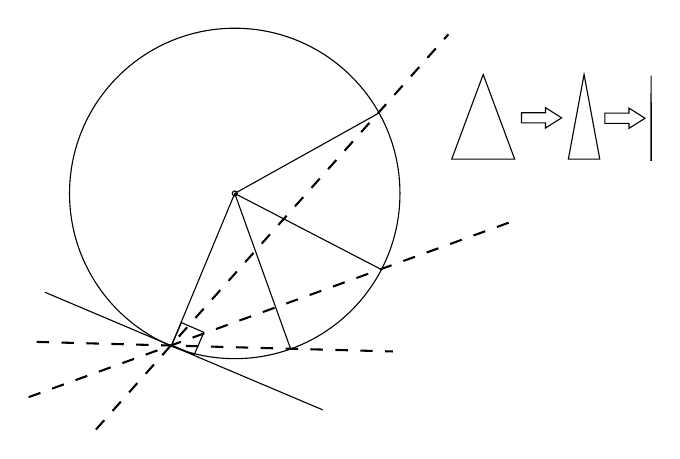
\begin{tikzpicture}[x=0.75pt,y=0.75pt,yscale=-.8,xscale=.8]
%uncomment if require: \path (0,300); %set diagram left start at 0, and has height of 300

%Shape: Circle [id:dp9462086222707395] 
\draw   (210.83,130.33) .. controls (210.83,75.38) and (255.38,30.83) .. (310.33,30.83) .. controls (365.29,30.83) and (409.83,75.38) .. (409.83,130.33) .. controls (409.83,185.29) and (365.29,229.83) .. (310.33,229.83) .. controls (255.38,229.83) and (210.83,185.29) .. (210.83,130.33) -- cycle ;
%Shape: Circle [id:dp047578291925302274] 
\draw   (308.83,130.33) .. controls (308.83,129.5) and (309.5,128.83) .. (310.33,128.83) .. controls (311.16,128.83) and (311.83,129.5) .. (311.83,130.33) .. controls (311.83,131.16) and (311.16,131.83) .. (310.33,131.83) .. controls (309.5,131.83) and (308.83,131.16) .. (308.83,130.33) -- cycle ;
%Straight Lines [id:da164533467123273] 
\draw    (310.33,130.33) -- (397,82) ;
%Straight Lines [id:da6876805606476655] 
\draw    (310.33,130.33) -- (399,176.33) ;
%Straight Lines [id:da2683999503020207] 
\draw    (310.33,130.33) -- (344,224) ;
%Straight Lines [id:da5819396491391264] 
\draw    (310.33,130.33) -- (272.33,221.67) ;
%Straight Lines [id:da526688893527204] 
\draw    (196,189.83) -- (363.33,260.67) ;
%Shape: Square [id:dp49735363204371774] 
\draw   (278.19,208.12) -- (291.73,213.98) -- (285.88,227.52) -- (272.33,221.67) -- cycle ;
%Straight Lines [id:da7088460943857118] 
\draw [line width=0.75]  [dash pattern={on 4.5pt off 4.5pt}]  (191,219.75) -- (405.5,225.5) ;
%Straight Lines [id:da7797532755668244] 
\draw [line width=0.75]  [dash pattern={on 4.5pt off 4.5pt}]  (186.25,253) -- (477.25,147.25) ;
%Straight Lines [id:da04071479399088074] 
\draw [line width=0.75]  [dash pattern={on 4.5pt off 4.5pt}]  (226.75,272.5) -- (439,34.5) ;
%Shape: Triangle [id:dp8516868808756333] 
\draw   (459.96,58.67) -- (478.92,109.67) -- (441,109.67) -- cycle ;
%Shape: Triangle [id:dp9288674500496883] 
\draw   (520.71,58.67) -- (530.17,109.67) -- (511.25,109.67) -- cycle ;
%Shape: Triangle [id:dp887898710535237] 
\draw   (561.08,59.42) -- (560.92,110.42) -- (561.25,110.42) -- cycle ;
%Right Arrow [id:dp7969460603432355] 
\draw   (483,81.73) -- (497.5,81.73) -- (497.5,78.67) -- (507.17,84.79) -- (497.5,90.92) -- (497.5,87.85) -- (483,87.85) -- cycle ;
%Right Arrow [id:dp10153549174619747] 
\draw   (533.25,81.98) -- (547.75,81.98) -- (547.75,78.92) -- (557.42,85.04) -- (547.75,91.17) -- (547.75,88.1) -- (533.25,88.1) -- cycle ;



\end{tikzpicture}

\end{minipage}
\\\\
By having a line intersect a circle at random, a triangle is made when connecting the points of intersection to the center of the circle. The interior angle that is made can then be measured to be, presumably, less than $90^{\circ}$ (when there are two points of intersection made). \\
By bringing one of the points of intersection closer to the other, the triangle created becomes thinner and thinner, until it becomes a line that has an interior angle of $90^{\circ}$, and thus becomes tangent to the circle (intersects the circle at 1 point, and at a  $90^{\circ}$ angle).

\pagebreak

\subsubsection{The length of tangents from a point to a circle are equal}




\begin{minipage}{0.2\linewidth}
\tikzset{every picture/.style={line width=0.75pt}} %set default line width to 0.75pt        

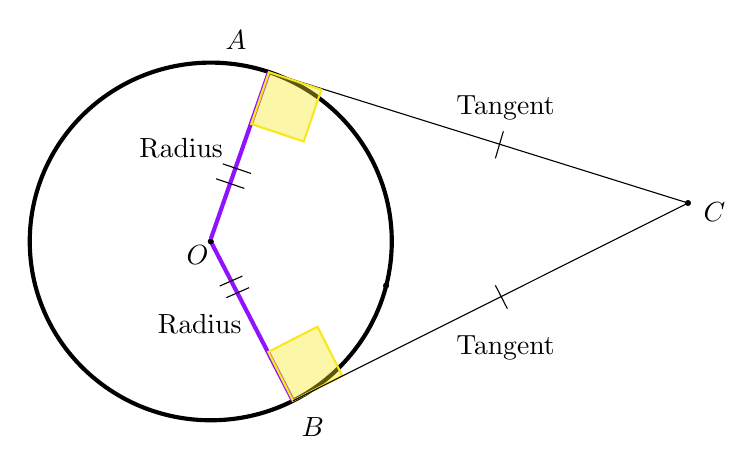
\begin{tikzpicture}[x=0.75pt,y=0.75pt,yscale=-0.8,xscale=0.8]
%uncomment if require: \path (0,419); %set diagram left start at 0, and has height of 419

%Shape: Ellipse [id:dp5403186956911956] 
\draw  [line width=1.5]  (121.97,174.07) .. controls (121.97,114.59) and (170.78,66.37) .. (230.99,66.37) .. controls (291.19,66.37) and (340,114.59) .. (340,174.07) .. controls (340,233.55) and (291.19,281.77) .. (230.99,281.77) .. controls (170.78,281.77) and (121.97,233.55) .. (121.97,174.07) -- cycle ;
%Straight Lines [id:da06811875685737068] 
\draw [color={rgb, 255:red, 144; green, 19; blue, 254 }  ,draw opacity=1 ][line width=1.5]    (230.99,174.07) -- (280.51,270.02) ;
%Shape: Ellipse [id:dp8767343798761416] 
\draw  [fill={rgb, 255:red, 0; green, 0; blue, 0 }  ,fill opacity=1 ] (229.52,174.07) .. controls (229.52,173.27) and (230.18,172.62) .. (230.99,172.62) .. controls (231.8,172.62) and (232.45,173.27) .. (232.45,174.07) .. controls (232.45,174.87) and (231.8,175.52) .. (230.99,175.52) .. controls (230.18,175.52) and (229.52,174.87) .. (229.52,174.07) -- cycle ;
%Shape: Ellipse [id:dp49749378737218897] 
\draw  [fill={rgb, 255:red, 0; green, 0; blue, 0 }  ,fill opacity=1 ] (335.07,200.67) .. controls (335.07,199.87) and (335.73,199.22) .. (336.54,199.22) .. controls (337.34,199.22) and (338,199.87) .. (338,200.67) .. controls (338,201.47) and (337.34,202.11) .. (336.54,202.11) .. controls (335.73,202.11) and (335.07,201.47) .. (335.07,200.67) -- cycle ;
%Straight Lines [id:da5760829311199731] 
\draw [color={rgb, 255:red, 144; green, 19; blue, 254 }  ,draw opacity=1 ][line width=1.5]    (266,72.13) -- (230.99,172.62) ;
%Straight Lines [id:da2529972826216105] 
\draw    (266,72.13) -- (518.4,150.93) ;
%Shape: Rectangle [id:dp2266551022394412] 
\draw  [color={rgb, 255:red, 248; green, 231; blue, 28 }  ,draw opacity=1 ][fill={rgb, 255:red, 248; green, 231; blue, 28 }  ,fill opacity=0.38 ][line width=0.75]  (265.62,240.62) -- (295.25,225.4) -- (310.13,254.81) -- (280.51,270.02) -- cycle ;
%Straight Lines [id:da9997015914374205] 
\draw    (280.51,270.02) -- (518.4,150.93) ;
%Shape: Ellipse [id:dp3407280289462833] 
\draw  [fill={rgb, 255:red, 0; green, 0; blue, 0 }  ,fill opacity=1 ] (516.93,150.93) .. controls (516.93,150.13) and (517.59,149.49) .. (518.4,149.49) .. controls (519.21,149.49) and (519.87,150.13) .. (519.87,150.93) .. controls (519.87,151.73) and (519.21,152.38) .. (518.4,152.38) .. controls (517.59,152.38) and (516.93,151.73) .. (516.93,150.93) -- cycle ;
%Straight Lines [id:da10566410471438958] 
\draw    (407.2,107.73) -- (402.4,124) ;
%Straight Lines [id:da6249154348250314] 
\draw    (402.4,200.53) -- (409.6,214.53) ;
%Straight Lines [id:da8015437869803181] 
\draw    (234.2,136.33) -- (251.2,142.13) ;
%Straight Lines [id:da2681549788104458] 
\draw    (236.4,200.93) -- (250,194.93) ;
%Straight Lines [id:da160461329674082] 
\draw    (240.4,207.93) -- (254,201.93) ;
%Straight Lines [id:da6992096843482827] 
\draw    (238.2,127.33) -- (255.2,133.13) ;
%Shape: Rectangle [id:dp24268413759610286] 
\draw  [color={rgb, 255:red, 248; green, 231; blue, 28 }  ,draw opacity=1 ][fill={rgb, 255:red, 248; green, 231; blue, 28 }  ,fill opacity=0.38 ][line width=0.75]  (266,72.13) -- (297.59,82.69) -- (286.96,113.88) -- (255.37,103.33) -- cycle ;

% Text Node
\draw (284.11,278.54) node [anchor=north west][inner sep=0.75pt]    {$B$};
% Text Node
\draw (526.2,148.91) node [anchor=north west][inner sep=0.75pt]    {$C$};
% Text Node
\draw (214.88,174.69) node [anchor=north west][inner sep=0.75pt]    {$O$};
% Text Node
\draw (197.56,216.1) node [anchor=north west][inner sep=0.75pt]   [align=left] {Radius};
% Text Node
\draw (377.28,229.32) node [anchor=north west][inner sep=0.75pt]   [align=left] {Tangent};
% Text Node
\draw (238.37,45.66) node [anchor=north west][inner sep=0.75pt]    {$A$};
% Text Node
\draw (186.36,110.5) node [anchor=north west][inner sep=0.75pt]   [align=left] {Radius};
% Text Node
\draw (377.28,84.52) node [anchor=north west][inner sep=0.75pt]   [align=left] {Tangent};


\end{tikzpicture}
\end{minipage}
\hfill
\begin{minipage}{0.35\linewidth}

Since $AO=BO$, OC is shared, and $\angle OAC=\angle OBC$ (SSA), $AC=BC$ (Hypotenuse Leg Theorem).
\end{minipage}

\vspace{100px}

\subsubsection{Tangent-Chord Theorem: the angle formed between a chord and a tangent line to a circle is equal to the inscribed angle on the other side of the chord}


\begin{minipage}{0.2\linewidth}




\tikzset{every picture/.style={line width=0.75pt}} %set default line width to 0.75pt        

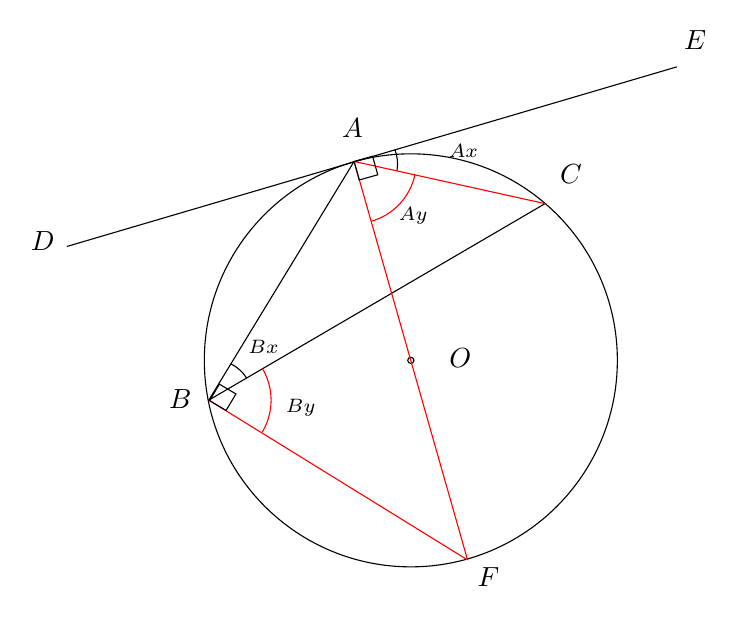
\begin{tikzpicture}[x=0.75pt,y=0.75pt,yscale=-1,xscale=1]
%uncomment if require: \path (0,300); %set diagram left start at 0, and has height of 300

%Shape: Circle [id:dp9462086222707395] 
\draw   (210.17,180.83) .. controls (210.17,125.88) and (254.71,81.33) .. (309.67,81.33) .. controls (364.62,81.33) and (409.17,125.88) .. (409.17,180.83) .. controls (409.17,235.79) and (364.62,280.33) .. (309.67,280.33) .. controls (254.71,280.33) and (210.17,235.79) .. (210.17,180.83) -- cycle ;
%Shape: Circle [id:dp047578291925302274] 
\draw   (308.17,180.83) .. controls (308.17,180) and (308.84,179.33) .. (309.67,179.33) .. controls (310.5,179.33) and (311.17,180) .. (311.17,180.83) .. controls (311.17,181.66) and (310.5,182.33) .. (309.67,182.33) .. controls (308.84,182.33) and (308.17,181.66) .. (308.17,180.83) -- cycle ;
%Straight Lines [id:da8877718960135994] 
\draw    (143.94,125.97) -- (437.81,39.44) ;
%Straight Lines [id:da14504871147163279] 
\draw    (282.33,85) -- (212.33,200) ;
%Straight Lines [id:da273202169691396] 
\draw    (212.33,200) -- (374.33,105.33) ;
%Straight Lines [id:da15786714847918626] 
\draw [color={rgb, 255:red, 255; green, 0; blue, 0 }  ,draw opacity=1 ]   (282.33,85) -- (374.33,105.33) ;
%Straight Lines [id:da30413004913216546] 
\draw [color={rgb, 255:red, 255; green, 0; blue, 0 }  ,draw opacity=1 ]   (282.33,85) -- (337,277) ;
%Straight Lines [id:da6346846203224932] 
\draw [color={rgb, 255:red, 255; green, 0; blue, 0 }  ,draw opacity=1 ]   (212.33,200) -- (337,277) ;
%Shape: Arc [id:dp43638639977515226] 
\draw  [draw opacity=0] (238.2,184.81) .. controls (241.77,190.89) and (243.23,198.24) .. (241.79,205.7) .. controls (241.1,209.24) and (239.82,212.51) .. (238.07,215.43) -- (212.33,200) -- cycle ; \draw  [color={rgb, 255:red, 255; green, 0; blue, 0 }  ,draw opacity=1 ] (238.2,184.81) .. controls (241.77,190.89) and (243.23,198.24) .. (241.79,205.7) .. controls (241.1,209.24) and (239.82,212.51) .. (238.07,215.43) ;  
%Shape: Arc [id:dp055476701941292506] 
\draw  [draw opacity=0] (222.95,182.5) .. controls (226.07,184.08) and (228.73,186.43) .. (230.59,189.39) -- (212.33,200) -- cycle ; \draw   (222.95,182.5) .. controls (226.07,184.08) and (228.73,186.43) .. (230.59,189.39) ;  
%Shape: Arc [id:dp4757574294397169] 
\draw  [draw opacity=0] (301.94,79.13) .. controls (303.2,82.4) and (303.59,85.93) .. (302.99,89.37) -- (282.33,85) -- cycle ; \draw   (301.94,79.13) .. controls (303.2,82.4) and (303.59,85.93) .. (302.99,89.37) ;  
%Shape: Arc [id:dp7955973919503874] 
\draw  [draw opacity=0] (311.66,91.3) .. controls (309.94,99.32) and (304.96,106.6) .. (297.29,111.01) .. controls (295.19,112.21) and (293,113.14) .. (290.78,113.79) -- (282.33,85) -- cycle ; \draw  [color={rgb, 255:red, 255; green, 0; blue, 0 }  ,draw opacity=1 ] (311.66,91.3) .. controls (309.94,99.32) and (304.96,106.6) .. (297.29,111.01) .. controls (295.19,112.21) and (293,113.14) .. (290.78,113.79) ;  
%Shape: Square [id:dp25354834815042304] 
\draw   (212.7,200.25) -- (217.43,192.29) -- (225.39,197.02) -- (220.66,204.98) -- cycle ;
%Shape: Square [id:dp9082911411710133] 
\draw   (282.33,85) -- (291.25,82.52) -- (293.73,91.44) -- (284.81,93.92) -- cycle ;

% Text Node
\draw (125.33,117.73) node [anchor=north west][inner sep=0.75pt]    {$D$};
% Text Node
\draw (440.08,20.82) node [anchor=north west][inner sep=0.75pt]    {$E$};
% Text Node
\draw (275.33,63.07) node [anchor=north west][inner sep=0.75pt]    {$A$};
% Text Node
\draw (380.33,85.4) node [anchor=north west][inner sep=0.75pt]    {$C$};
% Text Node
\draw (192,193.73) node [anchor=north west][inner sep=0.75pt]    {$B$};
% Text Node
\draw (327,174.07) node [anchor=north west][inner sep=0.75pt]    {$O$};
% Text Node
\draw (230.19,169.97) node [anchor=north west][inner sep=0.75pt]  [font=\scriptsize]  {$Bx$};
% Text Node
\draw (248.19,198.22) node [anchor=north west][inner sep=0.75pt]  [font=\scriptsize]  {$By$};
% Text Node
\draw (326.69,75.22) node [anchor=north west][inner sep=0.75pt]  [font=\scriptsize]  {$Ax$};
% Text Node
\draw (302.69,105.97) node [anchor=north west][inner sep=0.75pt]  [font=\scriptsize]  {$Ay$};
% Text Node
\draw (340.56,279.47) node [anchor=north west][inner sep=0.75pt]    {$F$};


\end{tikzpicture}


\end{minipage}
\hfill
\begin{minipage}{0.4\linewidth}
To prove that $\angle EAC$ is eqivalent to $\angle ABC$, draw a line from point A that passes through the center and intersects with the circumference of the circle. Since DE is tangent to the circle, $\angle EAF$ is  $90^{\circ}$. $\angle CBF$ is also  $90^{\circ}$, since $\angle CBF$ shares the same arc as $\angle EAF$ (ref. 1.4). \\
$\angle EAF$ can be considered as the sum of $Ax$ and $Ay$. We know that $By$ and $Ay$ are the same angle because the share the same arc. Thus, we know $Ax=Bx$, since  $90^{\circ}-Ay=$  $90^{\circ}-By=Ax=Bx$. 
\end{minipage}

\pagebreak

\section{Cyclic Quadrilateral (Four points cyclic)}

\subsection{Definition}
A quadrilateral which has all its four vertices lying on the perimeter of a circle.

\subsection{Opposite angles are added up to \(180^{\circ}\)}

\begin{minipage}{0.2\linewidth}

\tikzset{every picture/.style={line width=0.75pt}} %set default line width to 0.75pt        

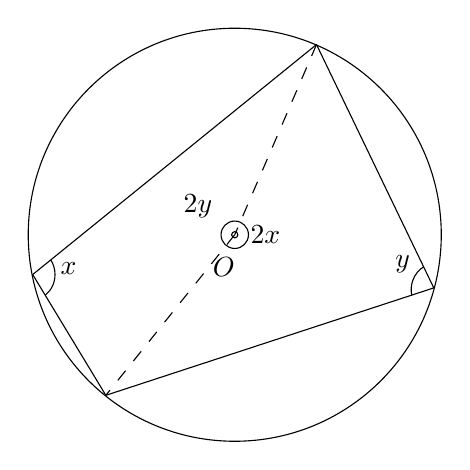
\begin{tikzpicture}[x=0.75pt,y=0.75pt,yscale=-1,xscale=1]
%uncomment if require: \path (0,300); %set diagram left start at 0, and has height of 300

%Shape: Circle [id:dp9462086222707395] 
\draw   (210.17,180.83) .. controls (210.17,125.88) and (254.71,81.33) .. (309.67,81.33) .. controls (364.62,81.33) and (409.17,125.88) .. (409.17,180.83) .. controls (409.17,235.79) and (364.62,280.33) .. (309.67,280.33) .. controls (254.71,280.33) and (210.17,235.79) .. (210.17,180.83) -- cycle ;
%Shape: Circle [id:dp047578291925302274] 
\draw   (308.17,180.83) .. controls (308.17,180) and (308.84,179.33) .. (309.67,179.33) .. controls (310.5,179.33) and (311.17,180) .. (311.17,180.83) .. controls (311.17,181.66) and (310.5,182.33) .. (309.67,182.33) .. controls (308.84,182.33) and (308.17,181.66) .. (308.17,180.83) -- cycle ;
%Straight Lines [id:da273202169691396] 
\draw    (212.33,200) -- (349.06,89.19) ;
%Straight Lines [id:da5600512377516604] 
\draw    (349.06,89.19) -- (405.56,206.44) ;
%Straight Lines [id:da21810832902148203] 
\draw    (247.56,258.19) -- (405.56,206.44) ;
%Straight Lines [id:da21582352436200725] 
\draw    (247.56,258.19) -- (212.33,200) ;
%Straight Lines [id:da4047868315915173] 
\draw  [dash pattern={on 4.5pt off 4.5pt}]  (309.67,180.83) -- (247.56,258.19) ;
%Straight Lines [id:da9433547871534407] 
\draw  [dash pattern={on 4.5pt off 4.5pt}]  (349.06,89.19) -- (309.67,180.83) ;
%Shape: Circle [id:dp8970580016855083] 
\draw   (303.06,180.83) .. controls (303.06,177.18) and (306.02,174.23) .. (309.67,174.23) .. controls (313.32,174.23) and (316.27,177.18) .. (316.27,180.83) .. controls (316.27,184.48) and (313.32,187.44) .. (309.67,187.44) .. controls (306.02,187.44) and (303.06,184.48) .. (303.06,180.83) -- cycle ;
%Shape: Arc [id:dp80004155117314] 
\draw  [draw opacity=0] (221.05,193) .. controls (222.32,194.97) and (223.07,197.39) .. (223.07,200) .. controls (223.07,204.11) and (221.22,207.74) .. (218.38,209.89) -- (212.33,200) -- cycle ; \draw   (221.05,193) .. controls (222.32,194.97) and (223.07,197.39) .. (223.07,200) .. controls (223.07,204.11) and (221.22,207.74) .. (218.38,209.89) ;  
%Shape: Arc [id:dp7002495093878305] 
\draw  [draw opacity=0] (394.96,209.98) .. controls (394.45,207.69) and (394.58,205.17) .. (395.49,202.71) .. controls (396.55,199.85) and (398.48,197.59) .. (400.8,196.19) -- (405.56,206.44) -- cycle ; \draw   (394.96,209.98) .. controls (394.45,207.69) and (394.58,205.17) .. (395.49,202.71) .. controls (396.55,199.85) and (398.48,197.59) .. (400.8,196.19) ;  

% Text Node
\draw (297.92,190.73) node [anchor=north west][inner sep=0.75pt]    {$O$};
% Text Node
\draw (283.81,160.22) node [anchor=north west][inner sep=0.75pt]    {$2y$};
% Text Node
\draw (316.06,175.22) node [anchor=north west][inner sep=0.75pt]    {$2x$};
% Text Node
\draw (224.56,192.97) node [anchor=north west][inner sep=0.75pt]    {$x$};
% Text Node
\draw (385.81,189.72) node [anchor=north west][inner sep=0.75pt]    {$y$};


\end{tikzpicture}

\end{minipage}
\hfill
\begin{minipage}{0.6\linewidth}
$2x+2y=360^\circ$\\
$(x+y)/2=360^\circ /2$\\
$x+y=180^\circ$
\end{minipage}
\subsection{How to prove four points cyclic}

\subsubsection{Prove these four points lies equally distance to another point — the center of the circle}

\subsubsection{Two equal angles subtend a segment (chord in the circle)}

\begin{minipage}{0.2\linewidth}


\tikzset{every picture/.style={line width=0.75pt}} %set default line width to 0.75pt        

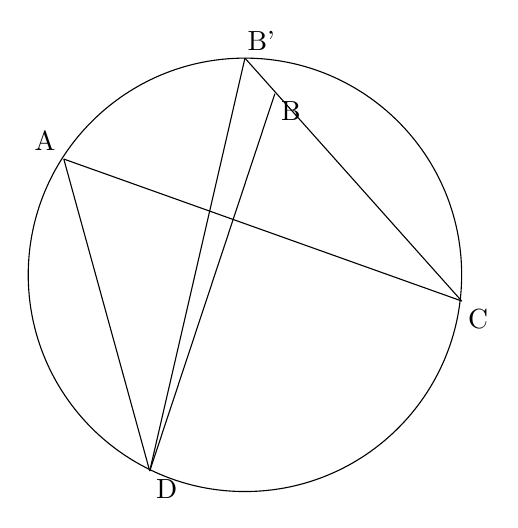
\begin{tikzpicture}[x=0.75pt,y=0.75pt,yscale=-.9,xscale=.9]
%uncomment if require: \path (0,411); %set diagram left start at 0, and has height of 411

%Shape: Circle [id:dp921091011277742] 
\draw   (125.97,202.01) .. controls (125.97,137.94) and (177.91,86) .. (241.99,86) .. controls (306.06,86) and (358,137.94) .. (358,202.01) .. controls (358,266.09) and (306.06,318.03) .. (241.99,318.03) .. controls (177.91,318.03) and (125.97,266.09) .. (125.97,202.01) -- cycle ;
%Straight Lines [id:da5459468360103272] 
\draw    (145.01,140.03) -- (191.01,307.03) ;
%Straight Lines [id:da588908423869051] 
\draw    (145.01,140.03) -- (358.01,216.03) ;
%Straight Lines [id:da0661291040591152] 
\draw    (258.01,105.03) -- (191.01,307.03) ;
%Straight Lines [id:da9044187873024561] 
\draw    (241.99,86) -- (358.01,216.03) ;
%Straight Lines [id:da12052154539862125] 
\draw    (241.99,86) -- (191.01,307.03) ;

% Text Node
\draw (128.01,124.03) node [anchor=north west][inner sep=0.75pt]   [align=left] {A};
% Text Node
\draw (260.01,108.03) node [anchor=north west][inner sep=0.75pt]   [align=left] {B};
% Text Node
\draw (360.01,219.03) node [anchor=north west][inner sep=0.75pt]   [align=left] {C};
% Text Node
\draw (193.01,310.03) node [anchor=north west][inner sep=0.75pt]   [align=left] {D};
% Text Node
\draw (241.99,70) node [anchor=north west][inner sep=0.75pt]   [align=left] {B'};


\end{tikzpicture}


\end{minipage}
\hfill
\begin{minipage}{0.55\linewidth}
If not, then let BC intersect circle at B'. \\
By 1.4, $\angle B'=\angle A$ \\
By Hypothesis, $\angle DBC = \angle A$ \\
Then $\angle BDB'=\angle B'-\angle DBC=0$ \\
Therefore, B and B' must be the same point.
\end{minipage}

\subsubsection{The sum of the opposite angle is $180^\circ$}

Proof is similar to 2.3.2
\pagebreak

\section{Similar triangles involving a circle}

\subsection{Identify as many similar triangles as possible}



\tikzset{every picture/.style={line width=0.75pt}} %set default line width to 0.75pt        

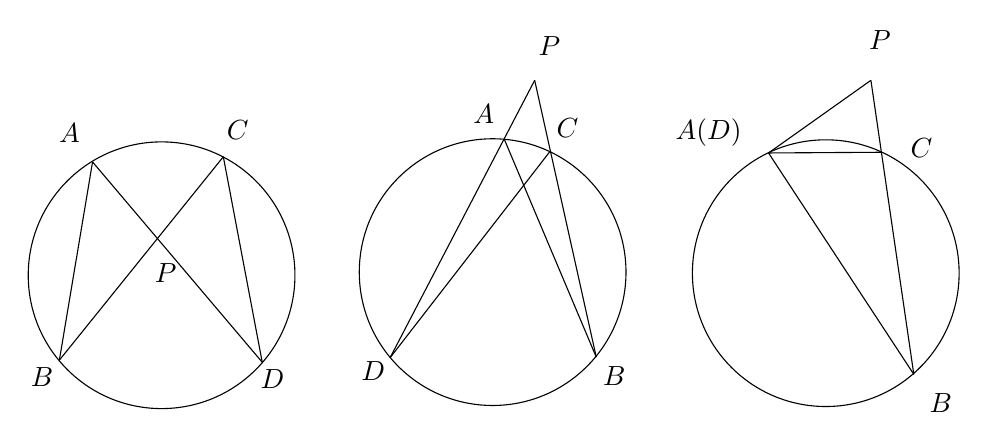
\begin{tikzpicture}[x=0.75pt,y=0.75pt,yscale=-1,xscale=1]
%uncomment if require: \path (0,300); %set diagram left start at 0, and has height of 300

%Shape: Circle [id:dp9462086222707395] 
\draw   (56,135.58) .. controls (56,100.1) and (84.77,71.33) .. (120.25,71.33) .. controls (155.73,71.33) and (184.5,100.1) .. (184.5,135.58) .. controls (184.5,171.07) and (155.73,199.83) .. (120.25,199.83) .. controls (84.77,199.83) and (56,171.07) .. (56,135.58) -- cycle ;
%Shape: Circle [id:dp2794602066066383] 
\draw   (215.5,134.08) .. controls (215.5,98.6) and (244.27,69.83) .. (279.75,69.83) .. controls (315.23,69.83) and (344,98.6) .. (344,134.08) .. controls (344,169.57) and (315.23,198.33) .. (279.75,198.33) .. controls (244.27,198.33) and (215.5,169.57) .. (215.5,134.08) -- cycle ;
%Shape: Circle [id:dp2098638970822193] 
\draw   (376,134.58) .. controls (376,99.1) and (404.77,70.33) .. (440.25,70.33) .. controls (475.73,70.33) and (504.5,99.1) .. (504.5,134.58) .. controls (504.5,170.07) and (475.73,198.83) .. (440.25,198.83) .. controls (404.77,198.83) and (376,170.07) .. (376,134.58) -- cycle ;
%Straight Lines [id:da5152896269286067] 
\draw    (87,81) -- (71,176.5) ;
%Straight Lines [id:da15239096947011244] 
\draw    (150,78.5) -- (71,176.5) ;
%Straight Lines [id:da25778811178108385] 
\draw    (87,81) -- (168.75,177.5) ;
%Straight Lines [id:da2120560799189919] 
\draw    (150,78.5) -- (168.75,177.5) ;
%Straight Lines [id:da44778435792701554] 
\draw    (230.33,175.33) -- (300,41.67) ;
%Straight Lines [id:da6755479195347789] 
\draw    (329.67,175) -- (300,41.67) ;
%Straight Lines [id:da6392213661182822] 
\draw    (307.33,76) -- (230.33,175.33) ;
%Straight Lines [id:da8530718760752225] 
\draw    (285.33,70) -- (329.67,175) ;
%Straight Lines [id:da6101067773970859] 
\draw    (412.67,76.67) -- (467.33,76.33) ;
%Straight Lines [id:da34512543218122715] 
\draw    (462,41.67) -- (482.67,183.33) ;
%Straight Lines [id:da9715744468004663] 
\draw    (462,41.67) -- (412.67,76.67) ;
%Straight Lines [id:da2338671063220683] 
\draw    (412.67,76.67) -- (482.67,183.33) ;

% Text Node
\draw (269.17,52.07) node [anchor=north west][inner sep=0.75pt]    {$A$};
% Text Node
\draw (331.67,178.4) node [anchor=north west][inner sep=0.75pt]    {$B$};
% Text Node
\draw (309.33,58.73) node [anchor=north west][inner sep=0.75pt]    {$C$};
% Text Node
\draw (215.25,175.98) node [anchor=north west][inner sep=0.75pt]    {$D$};
% Text Node
\draw (300.67,19.23) node [anchor=north west][inner sep=0.75pt]    {$P$};
% Text Node
\draw (366.67,58.73) node [anchor=north west][inner sep=0.75pt]    {$A( D)$};
% Text Node
\draw (489.08,191.48) node [anchor=north west][inner sep=0.75pt]    {$B$};
% Text Node
\draw (479.83,68.4) node [anchor=north west][inner sep=0.75pt]    {$C$};
% Text Node
\draw (459.83,16.57) node [anchor=north west][inner sep=0.75pt]    {$P$};
% Text Node
\draw (69.58,61.32) node [anchor=north west][inner sep=0.75pt]    {$A$};
% Text Node
\draw (56,178.73) node [anchor=north west][inner sep=0.75pt]    {$B$};
% Text Node
\draw (150.42,59.98) node [anchor=north west][inner sep=0.75pt]    {$C$};
% Text Node
\draw (166.67,179.57) node [anchor=north west][inner sep=0.75pt]    {$D$};
% Text Node
\draw (115.75,128.82) node [anchor=north west][inner sep=0.75pt]    {$P$};


\end{tikzpicture}


\vspace{40px}

\subsection{Power of a point}

\subsubsection{Definition:}
A real number that demonstrates the distance a point from a circle.

\subsubsection{Power of point is fixed regardless the choice of chord}

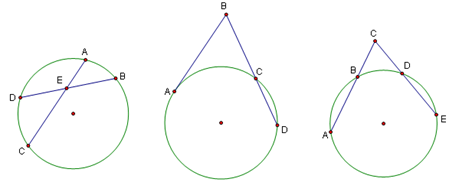
\includegraphics[scale=1.2]{Picture13.png}
\\
A ratio between the side lengths of the two similar triangles DEC and AEB can be made by having a fraction with one line over it's "pair". Therefore, for the first figure, $EA/DE=BE/CE\longrightarrow EA\times EC=BE\times DE$. As a result, the power of a point is the same for any two intersections made by a straight line from a single point. As a result, we can determine that $BA\times BA=BC\times BD$, and $CB\times CA=CD\times CE$, for figure 2 and 3 respectively.
\pagebreak

\subsubsection{Power of a point formula}

\[PoP = {PO}^2-r^2\]

\begin{center}
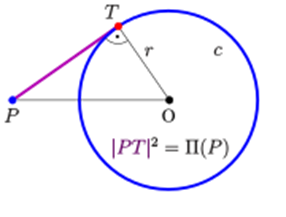
\includegraphics{Picture14.png}
\end{center}
We know that $PoP=PT^2$, and that PT is tangent to the circle, therefore making $\angle PTO=90^\circ$. We can then use the Pythagorean theorem, resulting in: $PT^2=PO^2-r^2$.
\vspace{60px}

\subsection{Homothety involving circles}

\subsubsection{Homothety of a circle is a circle}

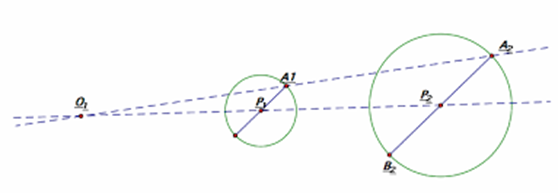
\includegraphics{Picture15.png}
\\
The ratio between the two circles can be displayed as a fraction: $OP_1/OP_2$. Therefore, $P_1A_1=R$, and $P_2A_2=R\times r$. 
\subsubsection{Ratios in the homothety}
$R/r$ is the ratio of homothety (ref. 3.3.1).
\pagebreak

\section{Problems}

\subsection{Problem}
Given AD AE are the internal, external angle bisector of angle A,
 such that D,E are the intersection of the angle bisectors with the circumcircle. 
 Prove DE is a diameter of the circle.

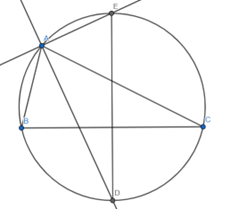
\includegraphics{Picture16.png}

Since $EAD =90^\circ$, $DE$ is a diameter of the circumcircle.
In addition, since $AD$ is the internal angle bisector,
$D$ is the midpoint of arc $AB$ as $\angle BAD = \angle CAD$.
Similarly, $E$ is the midpoint of arc $BAC$.

\subsection{Problem}
Given Circle C1, C2 intersect at A, B, CD is the common tangent to both circles, 
E is the intersection of AB and CD. Prove E is the midpoint of CD.
\\\\
\begin{minipage}{0.2\linewidth}
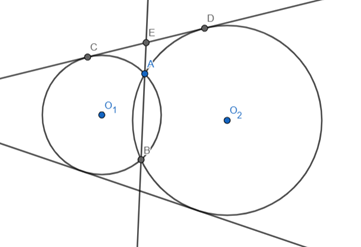
\includegraphics{Picture17.png}
\end{minipage}
\hfill
\begin{minipage}{0.35\linewidth}
$EC^2=EA\times EB$\\
$ED^2=EA\times EB$\\
Since, $EC^2=ED^2$\\
Therefore, $EC=ED$
\end{minipage}
\pagebreak

\subsection{Theorem}
In a triangle abc=4RS

\begin{minipage}{0.2\linewidth}


\tikzset{every picture/.style={line width=0.75pt}} %set default line width to 0.75pt        

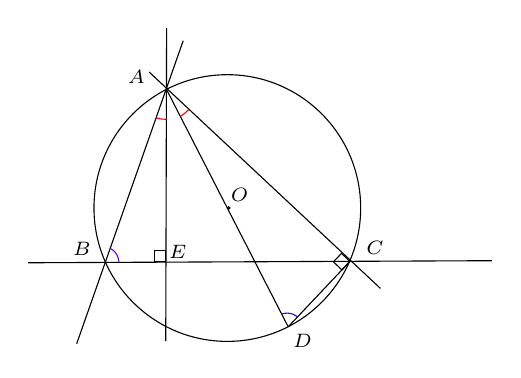
\begin{tikzpicture}[x=0.75pt,y=0.75pt,yscale=-1,xscale=1]
%uncomment if require: \path (0,300); %set diagram left start at 0, and has height of 300

%Shape: Circle [id:dp2794602066066383] 
\draw   (215.42,134.22) .. controls (215.42,98.74) and (244.18,69.97) .. (279.67,69.97) .. controls (315.15,69.97) and (343.92,98.74) .. (343.92,134.22) .. controls (343.92,169.71) and (315.15,198.47) .. (279.67,198.47) .. controls (244.18,198.47) and (215.42,169.71) .. (215.42,134.22) -- cycle ;
%Straight Lines [id:da562992416038582] 
\draw    (250.42,47.59) -- (250,198.33) ;
%Straight Lines [id:da7994376896201953] 
\draw    (242,68.67) -- (353.42,172.92) ;
%Straight Lines [id:da9295963036997694] 
\draw    (183.75,160.59) -- (407.09,159.59) ;
%Straight Lines [id:da06964743659693018] 
\draw [fill={rgb, 255:red, 183; green, 10; blue, 10 }  ,fill opacity=1 ]   (258.42,53.59) -- (207.09,199.59) ;
%Straight Lines [id:da5647560629982864] 
\draw    (250.33,77) -- (309,191.44) ;
%Straight Lines [id:da4600410665130259] 
\draw    (309,191.44) -- (338.75,159.94) ;
%Shape: Square [id:dp9549672722698885] 
\draw   (244.38,154.57) -- (250,154.57) -- (250,160.19) -- (244.38,160.19) -- cycle ;
%Shape: Square [id:dp8467083766989931] 
\draw   (330.8,160.14) -- (334.68,156.06) -- (338.75,159.94) -- (334.87,164.02) -- cycle ;
%Shape: Arc [id:dp13227288253715686] 
\draw  [draw opacity=0] (250.44,91.51) .. controls (250.4,91.51) and (250.37,91.51) .. (250.33,91.51) .. controls (248.6,91.51) and (246.93,91.27) .. (245.36,90.82) -- (250.33,77) -- cycle ; \draw  [color={rgb, 255:red, 255; green, 0; blue, 0 }  ,draw opacity=1 ] (250.44,91.51) .. controls (250.4,91.51) and (250.37,91.51) .. (250.33,91.51) .. controls (248.6,91.51) and (246.93,91.27) .. (245.36,90.82) ;  
%Shape: Arc [id:dp22862431958153073] 
\draw  [draw opacity=0] (261.12,86.71) .. controls (261.09,86.74) and (261.07,86.76) .. (261.05,86.79) .. controls (259.88,88.07) and (258.57,89.14) .. (257.18,89.99) -- (250.33,77) -- cycle ; \draw  [color={rgb, 255:red, 255; green, 0; blue, 0 }  ,draw opacity=1 ] (261.12,86.71) .. controls (261.09,86.74) and (261.07,86.76) .. (261.05,86.79) .. controls (259.88,88.07) and (258.57,89.14) .. (257.18,89.99) ;  
%Shape: Arc [id:dp596211273778789] 
\draw  [draw opacity=0] (223.48,153.78) .. controls (225.05,154.63) and (226.35,156.11) .. (227.02,158.03) .. controls (227.28,158.77) and (227.43,159.52) .. (227.46,160.25) -- (220.89,160.17) -- cycle ; \draw  [color={rgb, 255:red, 96; green, 0; blue, 255 }  ,draw opacity=1 ] (223.48,153.78) .. controls (225.05,154.63) and (226.35,156.11) .. (227.02,158.03) .. controls (227.28,158.77) and (227.43,159.52) .. (227.46,160.25) ;  
%Shape: Arc [id:dp37441445566940357] 
\draw  [draw opacity=0] (305.84,185.32) .. controls (307.5,184.68) and (309.48,184.65) .. (311.37,185.39) .. controls (312.1,185.68) and (312.76,186.06) .. (313.35,186.51) -- (309,191.44) -- cycle ; \draw  [color={rgb, 255:red, 49; green, 0; blue, 255 }  ,draw opacity=1 ] (305.84,185.32) .. controls (307.5,184.68) and (309.48,184.65) .. (311.37,185.39) .. controls (312.1,185.68) and (312.76,186.06) .. (313.35,186.51) ;  
%Shape: Circle [id:dp0198050007406807] 
\draw   (279.67,134.22) .. controls (279.67,133.88) and (279.95,133.6) .. (280.29,133.6) .. controls (280.63,133.6) and (280.91,133.88) .. (280.91,134.22) .. controls (280.91,134.56) and (280.63,134.84) .. (280.29,134.84) .. controls (279.95,134.84) and (279.67,134.56) .. (279.67,134.22) -- cycle ;

% Text Node
\draw (230.64,66.68) node [anchor=north west][inner sep=0.75pt]  [font=\scriptsize]  {$A$};
% Text Node
\draw (280.14,123.43) node [anchor=north west][inner sep=0.75pt]  [font=\scriptsize]  {$O$};
% Text Node
\draw (345.39,148.93) node [anchor=north west][inner sep=0.75pt]  [font=\scriptsize]  {$C$};
% Text Node
\draw (250.39,150.93) node [anchor=north west][inner sep=0.75pt]  [font=\scriptsize]  {$E$};
% Text Node
\draw (204.14,149.68) node [anchor=north west][inner sep=0.75pt]  [font=\scriptsize]  {$B$};
% Text Node
\draw (310.14,193.93) node [anchor=north west][inner sep=0.75pt]  [font=\scriptsize]  {$D$};


\end{tikzpicture}

\end{minipage}
\hfill
\begin{minipage}{0.5\linewidth}
We know $\triangle AEB$ is similar to $\triangle ACD$, since $\angle BAE=\angle DAC$ ($\angle ABC=\angle ADC$ since they share the same arc, and AE is perpendicular to EB, similar to how AC is perpendicular to DC).\\
Therefore, we can state $AE/AB=AC/AD\longrightarrow AE\times 2r=AC\times AB=bc$.\\
Finally, $abc=2R\times AE\times a=4R\times (\frac{AE\times BC}{2})=4RS$, where S is the area of ABC

\end{minipage}

\subsection{Problem}

Given AE is the external angle bisector of angle A, 
AE intersects BC at G, 
the tangent at A intersects BC at F. 
Prove AFG is an isosceles triangle.



\tikzset{every picture/.style={line width=0.75pt}} %set default line width to 0.75pt        

\begin{tikzpicture}[x=0.75pt,y=0.75pt,yscale=-1.6,xscale=1.6]
%uncomment if require: \path (0,300); %set diagram left start at 0, and has height of 300

%Shape: Circle [id:dp2794602066066383] 
\draw   (215.42,134.22) .. controls (215.42,98.74) and (244.18,69.97) .. (279.67,69.97) .. controls (315.15,69.97) and (343.92,98.74) .. (343.92,134.22) .. controls (343.92,169.71) and (315.15,198.47) .. (279.67,198.47) .. controls (244.18,198.47) and (215.42,169.71) .. (215.42,134.22) -- cycle ;
%Straight Lines [id:da9295963036997694] 
\draw    (75.5,160) -- (407.09,159.59) ;
%Straight Lines [id:da04780946384530149] 
\draw    (230,93.25) -- (221,159.75) ;
%Straight Lines [id:da582836471963158] 
\draw    (230,93.25) -- (338.75,160) ;
%Straight Lines [id:da29944212726334096] 
\draw    (230,93.25) -- (297.75,228.75) ;
%Straight Lines [id:da48123026856809825] 
\draw    (314,48.25) -- (91.75,167.5) ;
%Straight Lines [id:da3072783140413484] 
\draw    (275.75,33.5) -- (140,210.75) ;
%Shape: Arc [id:dp24987469828003062] 
\draw  [draw opacity=0] (329,160) .. controls (329,160) and (329,160) .. (329,160) .. controls (329,158.13) and (329.56,156.38) .. (330.51,154.91) -- (338.75,160) -- cycle ; \draw   (329,160) .. controls (329,160) and (329,160) .. (329,160) .. controls (329,158.13) and (329.56,156.38) .. (330.51,154.91) ;  
%Shape: Arc [id:dp2781603508357975] 
\draw  [draw opacity=0] (224.77,101.48) .. controls (224.77,101.48) and (224.77,101.48) .. (224.77,101.48) .. controls (223.19,100.47) and (222.01,99.07) .. (221.29,97.47) -- (230,93.25) -- cycle ; \draw   (224.77,101.48) .. controls (224.77,101.48) and (224.77,101.48) .. (224.77,101.48) .. controls (223.19,100.47) and (222.01,99.07) .. (221.29,97.47) ;  

% Text Node
\draw (219.14,80.93) node [anchor=north west][inner sep=0.75pt]  [font=\scriptsize]  {$A$};
% Text Node
\draw (343.14,146.93) node [anchor=north west][inner sep=0.75pt]  [font=\scriptsize]  {$C$};
% Text Node
\draw (272.39,71.43) node [anchor=north west][inner sep=0.75pt]  [font=\scriptsize]  {$E$};
% Text Node
\draw (223.89,147.18) node [anchor=north west][inner sep=0.75pt]  [font=\scriptsize]  {$B$};
% Text Node
\draw (282.39,185.68) node [anchor=north west][inner sep=0.75pt]  [font=\scriptsize]  {$D$};
% Text Node
\draw (172.89,147.43) node [anchor=north west][inner sep=0.75pt]  [font=\scriptsize]  {$F$};
% Text Node
\draw (100.14,145.18) node [anchor=north west][inner sep=0.75pt]  [font=\scriptsize]  {$G$};
% Text Node
\draw (219.75,108.15) node [anchor=north west][inner sep=0.75pt]  [font=\tiny]  {$y$};
% Text Node
\draw (241.75,89.65) node [anchor=north west][inner sep=0.75pt]  [font=\tiny]  {$x$};
% Text Node
\draw (317,150.15) node [anchor=north west][inner sep=0.75pt]  [font=\tiny]  {$y$};
% Text Node
\draw (189,114.15) node [anchor=north west][inner sep=0.75pt]  [font=\tiny]  {$x-y$};
% Text Node
\draw (120.25,153.4) node [anchor=north west][inner sep=0.75pt]  [font=\tiny]  {$x-y$};


\end{tikzpicture}
\\\\
Since $AE$ is the external angle bisector, $\angle GAB= \angle EAC$.\\
Also, by Tangent-Chord Theorem, $\angle FAB = \angle ACB$. \\
Therefore, $\angle G = \angle EAC - \angle ACB = \angle GAB - \angle FAB = \angle GAF$ (External Angle Theorem), and thus, AFG is an isosceles triangle.

\pagebreak

\subsection{Ptolemy's theorem}
If a quadrilateral is inscribed in a circle then the product of the lengths of its diagonals is equal to the sum of the products of the lengths of the pairs of opposite sides.
\\Or ab+cd=xy where a,b,c,d are the sides of the quadrilateral and x,y are the diagonals.\\
\begin{center}
\tikzset{every picture/.style={line width=0.75pt}} %set default line width to 0.75pt        

\begin{tikzpicture}[x=0.75pt,y=0.75pt,yscale=-1.6,xscale=1.6]
%uncomment if require: \path (0,300); %set diagram left start at 0, and has height of 300

%Shape: Ellipse [id:dp2794602066066383] 
\draw   (262.15,125.49) .. controls (262.15,77.72) and (301.03,39) .. (349,39) .. controls (396.97,39) and (435.86,77.72) .. (435.86,125.49) .. controls (435.86,173.25) and (396.97,211.97) .. (349,211.97) .. controls (301.03,211.97) and (262.15,173.25) .. (262.15,125.49) -- cycle ;
%Straight Lines [id:da9295963036997694] 
\draw    (147.25,160) -- (480.75,160) ;
%Straight Lines [id:da9694228198901165] 
\draw    (269.35,159.85) -- (321.06,43.41) ;
%Straight Lines [id:da4602575786504073] 
\draw    (435.86,125.49) -- (321.06,43.41) ;
%Straight Lines [id:da9298960848238496] 
\draw    (435.86,125.49) -- (269.35,159.85) ;
%Straight Lines [id:da520223449903894] 
\draw    (428.76,159.81) -- (321.06,43.41) ;
%Straight Lines [id:da36761229289035535] 
\draw    (321.06,43.41) -- (222.38,159.51) ;
%Straight Lines [id:da8712946570592159] 
\draw    (428.76,159.81) -- (435.86,125.49) ;

% Text Node
\draw (253.64,160.68) node [anchor=north west][inner sep=0.75pt]  [font=\normalsize]  {$A$};
% Text Node
\draw (428.14,161.93) node [anchor=north west][inner sep=0.75pt]  [font=\normalsize]  {$C$};
% Text Node
\draw (304.14,24.93) node [anchor=north west][inner sep=0.75pt]  [font=\normalsize]  {$B$};
% Text Node
\draw (435.89,110.43) node [anchor=north west][inner sep=0.75pt]  [font=\normalsize]  {$D$};
% Text Node
\draw (364.39,100.68) node [anchor=north west][inner sep=0.75pt]  [font=\scriptsize]  {$x$};
% Text Node
\draw (421.14,134.93) node [anchor=north west][inner sep=0.75pt]  [font=\scriptsize]  {$b$};
% Text Node
\draw (296.14,101.18) node [anchor=north west][inner sep=0.75pt]  [font=\scriptsize]  {$a$};
% Text Node
\draw (250.14,102.68) node [anchor=north west][inner sep=0.75pt]  [font=\scriptsize]  {$z$};
% Text Node
\draw (360.39,139.18) node [anchor=north west][inner sep=0.75pt]  [font=\scriptsize]  {$y$};
% Text Node
\draw (344.14,160.68) node [anchor=north west][inner sep=0.75pt]  [font=\scriptsize]  {$c$};
% Text Node
\draw (376.64,68.68) node [anchor=north west][inner sep=0.75pt]  [font=\scriptsize]  {$d$};
% Text Node
\draw (232.64,161.43) node [anchor=north west][inner sep=0.75pt]  [font=\scriptsize]  {$w$};
% Text Node
\draw (207.64,161.18) node [anchor=north west][inner sep=0.75pt]  [font=\normalsize]  {$E$};


\end{tikzpicture}
\end{center}

First, draw a reference line between point B that intersects the extended line AC with the same angle as $\angle DBC$ and label this point E. We know that $\triangle BEA$ is similar to $\triangle BCD$, and since they both share $\angle ABC$, $\triangle EBC$ is similar to $\triangle ABD$. Thus, we can create equivalent ratios with the various side lengths available:
$$\frac{z}{x}=\frac{a}{d}=\frac{w}{b}\Longrightarrow ab=wd$$\\
Since $\triangle BEC$ is similar to $\triangle BAD$,
$$\frac{z}{a}=\frac{x}{d}=\frac{w+c}{y}$$
$$wd+cd=xy$$
$$ab+cd=xy$$


\pagebreak

\subsection{Problem}
In \(\triangle\)ABC, point D is inside of ABC such that \(\angle \mathrm{DAC} = \angle \mathrm{DCA}=30^{\circ} \) and \(\angle \mathrm{DBA}=60^{\circ}\). E is the midpoint on BC and F is a trisect point on AC such that \(\mathrm{CF} = \frac{\mathrm{CA}}{3} \). Prove DE \(\perp\) EF.



\tikzset{every picture/.style={line width=0.75pt}} %set default line width to 0.75pt        

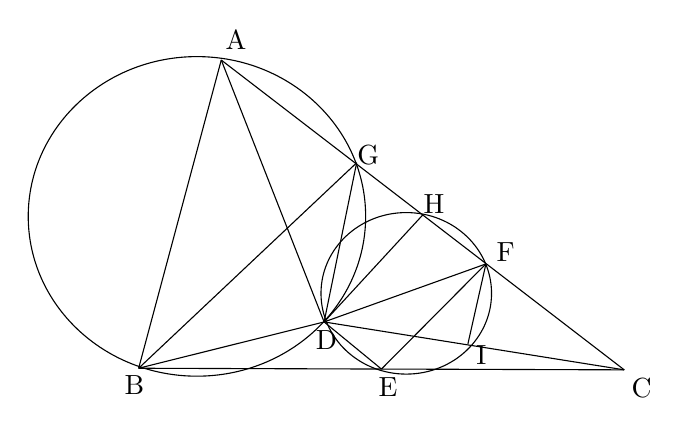
\begin{tikzpicture}[x=0.75pt,y=0.75pt,yscale=-.7,xscale=.7]
%uncomment if require: \path (0,300); %set diagram left start at 0, and has height of 300

%Straight Lines [id:da795234166630395] 
\draw    (219.43,37.61) -- (496.79,250.84) ;
%Straight Lines [id:da2470680087714714] 
\draw    (162.57,249.74) -- (496.79,250.84) ;
%Straight Lines [id:da7469666194240066] 
\draw    (219.43,37.61) -- (162.57,249.74) ;
%Straight Lines [id:da8315290951418923] 
\draw    (312.62,108.32) -- (162.57,249.74) ;
%Straight Lines [id:da27413735236355286] 
\draw    (312.62,108.32) -- (290.22,217.87) ;
%Straight Lines [id:da4498983652658053] 
\draw    (401.59,177.93) -- (290.22,217.87) ;
%Straight Lines [id:da12015425835999238] 
\draw    (290.22,217.87) -- (162.57,249.74) ;
%Straight Lines [id:da19572259445679085] 
\draw    (496.79,250.84) -- (290.22,217.87) ;
%Straight Lines [id:da1388174928028587] 
\draw    (389.21,232.89) -- (401.59,177.93) ;
%Straight Lines [id:da7036788173420365] 
\draw    (290.22,217.87) -- (329.68,250.29) ;
%Straight Lines [id:da7821068872992052] 
\draw    (219.43,37.61) -- (290.22,217.87) ;
%Straight Lines [id:da3718621800799] 
\draw    (358.11,144.23) -- (290.22,217.87) ;
%Straight Lines [id:da5614628174268017] 
\draw    (401.59,177.93) -- (329.68,250.29) ;
%Shape: Ellipse [id:dp47620171285324453] 
\draw   (86.57,145.22) .. controls (86.57,84.48) and (138.56,35.24) .. (202.69,35.24) .. controls (266.82,35.24) and (318.81,84.48) .. (318.81,145.22) .. controls (318.81,205.96) and (266.82,255.2) .. (202.69,255.2) .. controls (138.56,255.2) and (86.57,205.96) .. (86.57,145.22) -- cycle ;
%Shape: Ellipse [id:dp6903666392287857] 
\draw   (288.07,198.18) .. controls (288.07,167.48) and (314.35,142.59) .. (346.77,142.59) .. controls (379.18,142.59) and (405.46,167.48) .. (405.46,198.18) .. controls (405.46,228.88) and (379.18,253.77) .. (346.77,253.77) .. controls (314.35,253.77) and (288.07,228.88) .. (288.07,198.18) -- cycle ;

% Text Node
\draw (220.71,15.71) node [anchor=north west][inner sep=0.75pt]   [align=left] {A};
% Text Node
\draw (151.09,252.76) node [anchor=north west][inner sep=0.75pt]   [align=left] {B};
% Text Node
\draw (500.15,254.98) node [anchor=north west][inner sep=0.75pt]   [align=left] {C};
% Text Node
\draw (282.69,222.35) node [anchor=north west][inner sep=0.75pt]   [align=left] {D};
% Text Node
\draw (325.93,254.22) node [anchor=north west][inner sep=0.75pt]   [align=left] {E};
% Text Node
\draw (407.09,161.53) node [anchor=north west][inner sep=0.75pt]   [align=left] {F};
% Text Node
\draw (311.39,94.48) node [anchor=north west][inner sep=0.75pt]   [align=left] {G};
% Text Node
\draw (356.96,128.19) node [anchor=north west][inner sep=0.75pt]   [align=left] {H};
% Text Node
\draw (393.19,232.63) node [anchor=north west][inner sep=0.75pt]   [align=left] {I};


\end{tikzpicture}
\\
Let G be the midpoint of AF, Draw DH perpendicular to AC, FI perpendicular to CD.
Connect DG,DF,BG\\
\\
Claim 1: DFG is an equilateral triangle and AGD and DFC are 30-120-30 triangles.\\
Proof of Claim 1:\\
Let DC=x.\\
Since $\angle DAC = \angle DCA = 30^\circ$\\
$DH=\frac{x}{2}$, $CH = \frac{\sqrt{3}x}{2}$, $HF = \frac{HC}{3}$\\
Therefore, $HF = \frac{\sqrt{3}x}{6} = \frac{DH}{\sqrt{3}}$\\
This implies that DHF is a 30-60-90 triangle and DFC is a 30-120-30 triangle.\\
Similarly, AGD is a 30-120-30 triangle and therefore DFG is an equilateral triangle.\\
\\
By Claim 1, AGDB concyclic since $\angle ABD = \angle FGD = 60^\circ$\\
Also by Claim 1, I is the midpoint of CD.\\
\\
Now, consider the homothety from C with ratio 1/2.\\
It is clear that A maps to H, B maps to E, D maps to I, G maps to F.
Therefore, Circle ABDG maps to the circle HEIF (Note we haven't proved that D also lies on the same circle).\\
\\
Now, let's prove that D also lies on the same circle.\\
Since $\angle FDI = 30^\circ$, enough to show the arc IF = $60^\circ$ (arc is measured by the central angle).\\
However, by homothety, the measure of arc IF is the same as the measure of arc DG = $60^\circ$ as $\angle DAG =30^\circ$\\
Therefore, D lies in the circle HEIF or HDEIF concyclic.\\
\\
Since HDEIF concyclic, $\angle DEF=\angle DIF = 90^\circ$\\
Therefore, DE \(\perp\) EF.\\
Q.E.D.

\end{document}
